\section{measurement verse theory}

The aim of this section is to compare the result with the the analytical model and the simulation. This section will not evaluate the filters and therefore the evaluation will be done relative to \SI{0}{\decibel} at the front of the array. The performance of the filter and therefore also the absolute \gls{spl} will be evaluated in \autoref{sec:beamforming_array_spl}. All polar plot in \autoref{the_simulation_result} are converted to relative value, where the maximum value is the reference. The resend to use the maximum value and not the main axis of the speaker array is that the measurement have some asymmetric do to hardware error and therefore the highest pressure might not be exact on the main axis. 



 \begin{figure}[H]
	\centering
	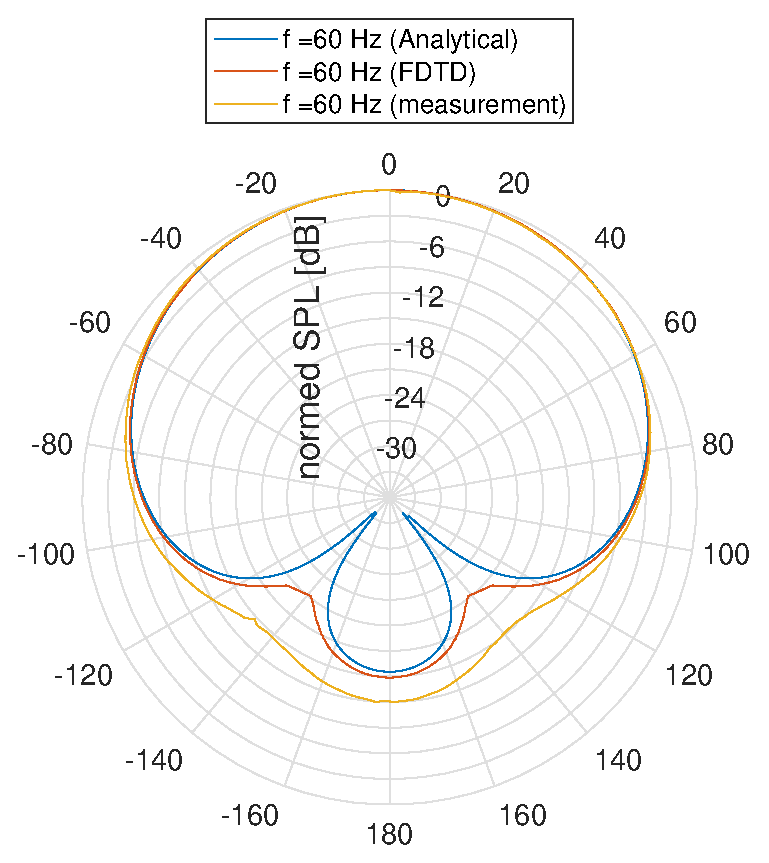
\includegraphics[width=1\textwidth]{60_hz_polar_result.eps}
	\caption{The figure shows}
		\label{fig:60_hz_polar_result}
\end{figure}

 \begin{figure}[H]
	\centering
	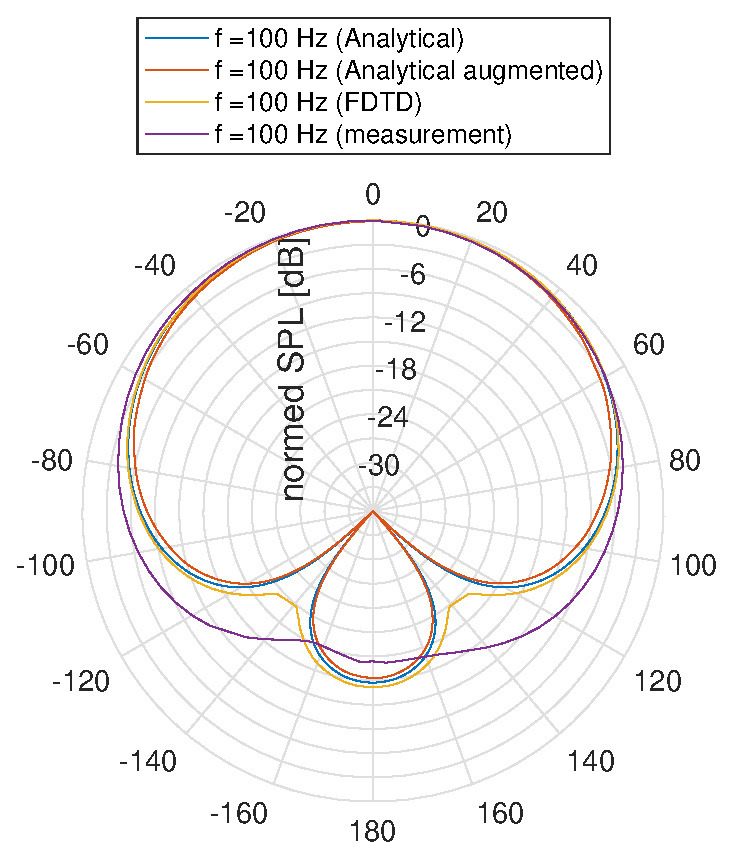
\includegraphics[width=1\textwidth]{100_hz_polar_result.eps}
	\caption{The figure shows}
		\label{fig:100_hz_polar_result}
\end{figure}

 \begin{figure}[H]
	\centering
	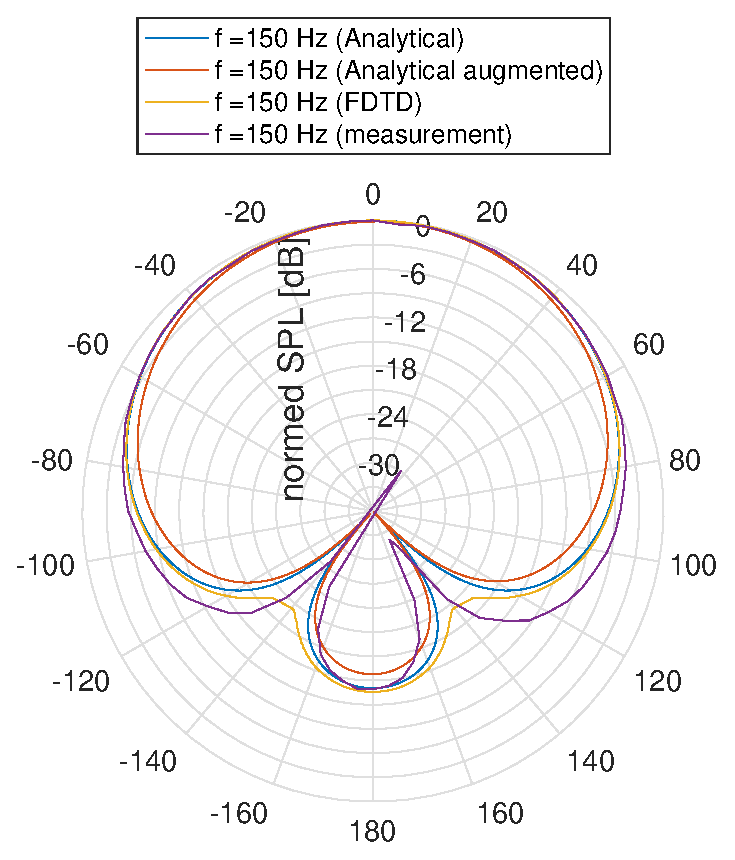
\includegraphics[width=1\textwidth]{150_hz_polar_result.eps}
	\caption{The figure shows}
		\label{fig:150_hz_polar_result}
\end{figure}

 \begin{figure}[H]
	\centering
	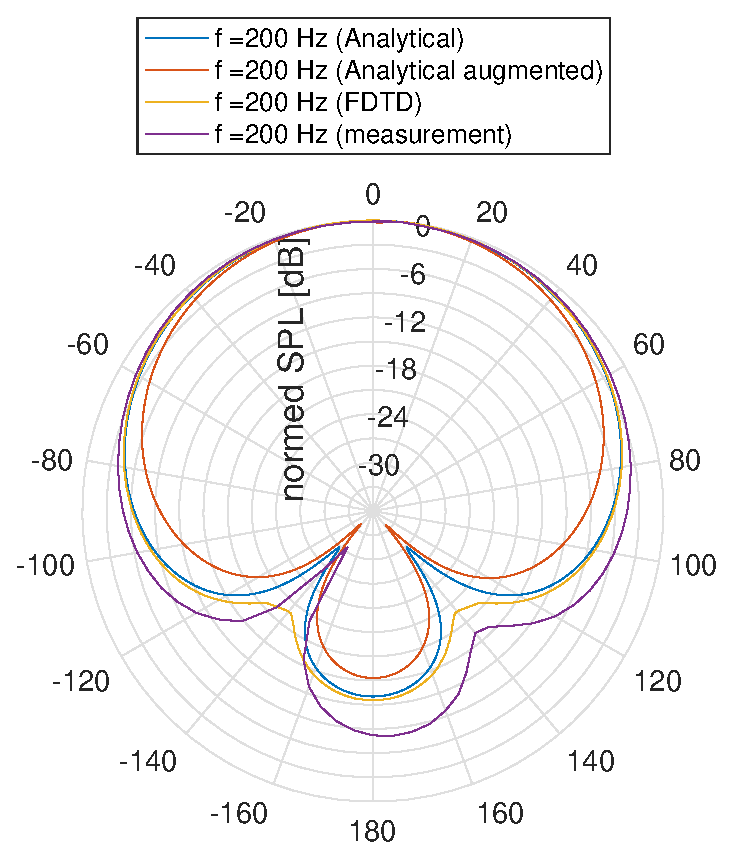
\includegraphics[width=1\textwidth]{200_hz_polar_result.eps}
	\caption{The figure shows}
		\label{fig:200_hz_polar_result}
\end{figure}


 \begin{figure}[H]
	\centering
	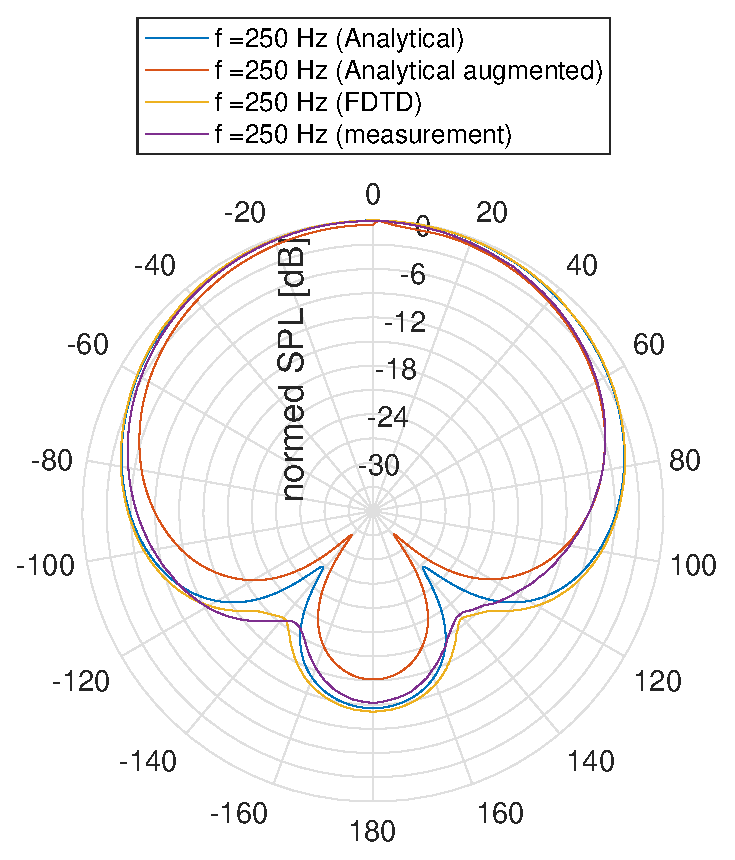
\includegraphics[width=1\textwidth]{250_hz_polar_result.eps}
	\caption{The figure shows}
		\label{fig:250_hz_polar_result}
\end{figure}

 \begin{figure}[H]
	\centering
	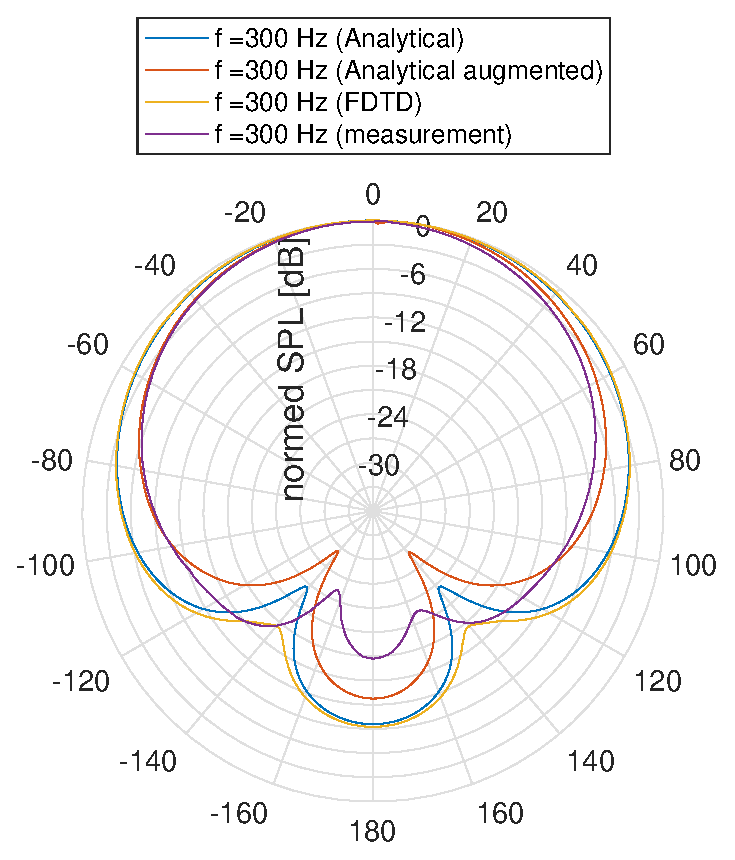
\includegraphics[width=1\textwidth]{300_hz_polar_result.eps}
	\caption{The figure shows}
		\label{fig:300_hz_polar_result}
\end{figure}







